
\documentclass[12pt]{beamer}

\usepackage[white]{beamerthemeWisconsin}
\usepackage{framed}
\usepackage{tikz}
%\usetheme[white]{Wisconsin}
\graphicspath{{./}{./uw-beamer-template/}}
\title{Leveraging Intel's Embree Ray Tracing in the DAGMC Toolkit}
\author{Patrick C Shriwise}
\institute{University of Wisconsin - Madison}
\date{ANS Winter Meeting 2015}




\AtBeginSection[]{
  \begin{frame}
  \vfill
  \centering
  \begin{beamercolorbox}[sep=8pt,center,shadow=true,rounded=true]{title}
    \usebeamerfont{title}\insertsectionhead\par%
  \end{beamercolorbox}
  \vfill
  \end{frame}
}


%%%% TIKZ OBJECTS %%%%
\usetikzlibrary{shapes.arrows}
\usetikzlibrary{positioning}
\usetikzlibrary{decorations.pathreplacing}

\tikzstyle{arrow} = [thick,->,>=stealth]

\tikzset{
    myarrow/.style={
        draw,
        fill=UWRed,
        single arrow,
        minimum height=4ex,
        single arrow head extend=1ex
    }
}

\newcommand{\arrowup}{%
\tikz [baseline=-0.5ex]{\node [myarrow,rotate=90] {};}
}
\newcommand{\arrowdown}{%
\tikz [baseline=-1ex]{\node [myarrow,rotate=-90] {};}
}
\newcommand{\arrowright}{%
\tikz [baseline=-0.5ex]{\node [myarrow,rotate=0] {};}
}
\newcommand{\doublearrow}{%
\tikz [baseline=-1ex]{\node [mydoublearrow,rotate=0] {};}
}



%%%% START DOCUMENT %%%%
\begin{document}


%% Title Frame %%
\frame{\titlepage \addtocounter{framenumber}{-1}}


%%Outline%%
\begin{frame}
\frametitle{\null}
\tableofcontents
\end{frame}

%% Introduction %%
\section{CAD-Based Monte Carlo Transport} % 1-2 slides
% We use it for our geometric queries:
   % point-inclusion
   % dist to next surf
% Replaces analytic intersections in native MonteCarlo packages
% Motivation: takes too long!
% Images of typical production models?
\begin{frame}

\frametitle{Robust CAD-Based Monte Carlo Transport}

DAGMC can robustly do transport calculations on models like these:


\begin{center}
\begin{tabular}{c c}

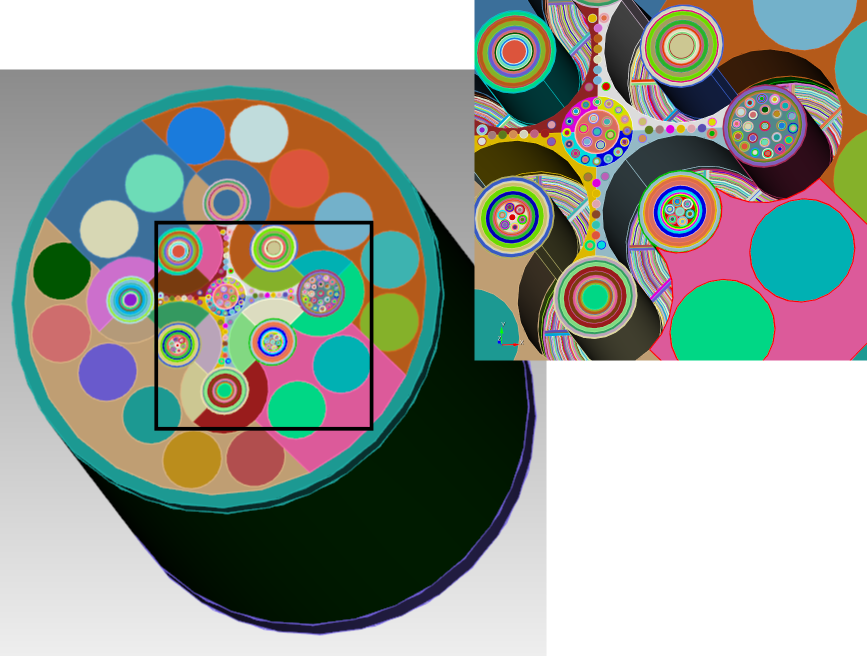
\includegraphics[height=0.4\textheight]{./images/atr_both.png} &
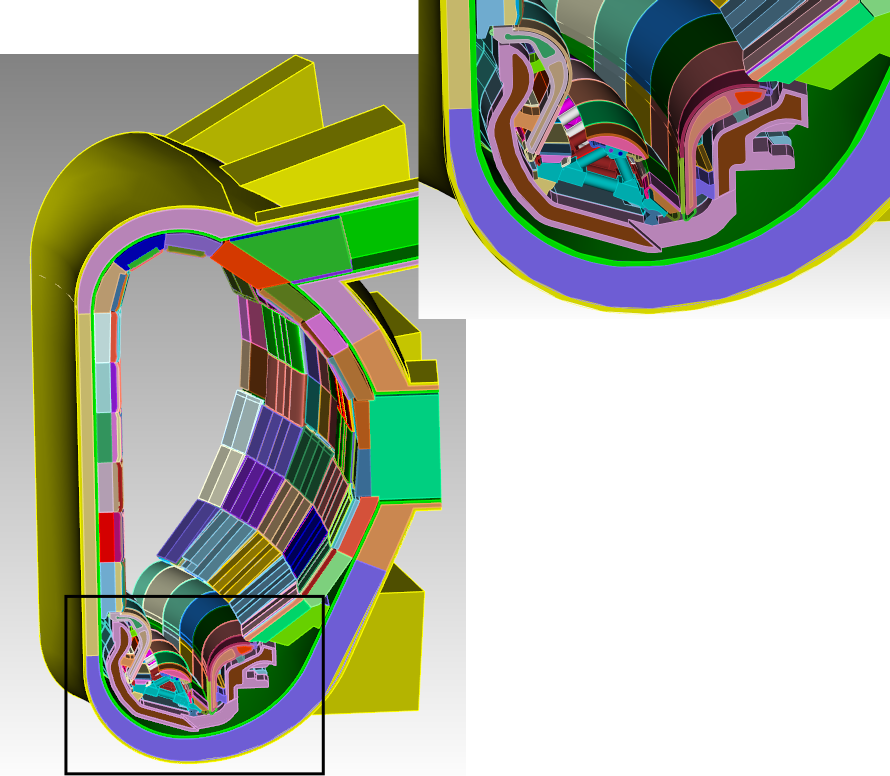
\includegraphics[height=0.4\textheight]{./images/bllite_both.png} \\

Advanced Test Reactor &
ITER \\

\end{tabular}
\end{center}

But it takes a long time... (2-10x slower than native codes)

\end{frame}

\begin{frame}

\frametitle{Ray Tracing in DAGMC}

\begin{itemize}
  \item Used for our geometric queries:
    \begin{itemize}
      \item point-inclusion tests
      \item next surface distance determination
    \end{itemize}
\end{itemize}


\end{frame}

\section{Ray Tracing Accelerations} % 2-3 slides
% BVH explanation in 1 slide
% Embree's tricks
% Extra: SAH


\begin{frame}
\frametitle{Bounding Volume Hierarchies}

\begin{itemize}
  \item By partitioning the geometry-based mesh using bounding volumes, we gain significant accelerations over a linear search of the discrete elements.
\end{itemize}

\begin{columns}
  \column{0.5\textwidth}
  \begin{figure}
    \centering
    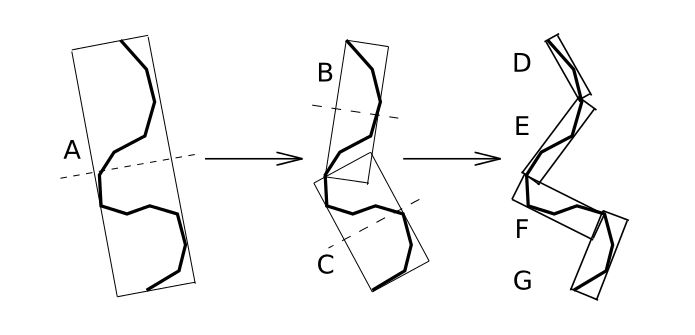
\includegraphics[width=1.1\textwidth]{./images/bvh_2d_ex_w_labels.png} 
    \cite{gottschalk1996obbtree}
  \end{figure}
  
  \column{0.4\textwidth}
  \begin{figure}
    \centering
    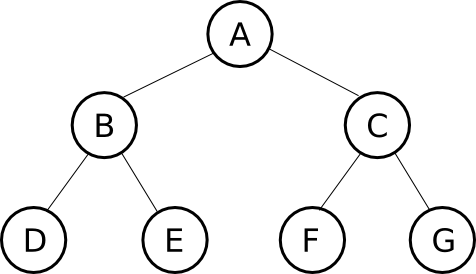
\includegraphics[width=0.5\textwidth]{./images/binary_graph.png}
  \end{figure}
\end{columns}

\vfill

\begin{itemize}
  \item How we create these hierarchies matters \textbf{a lot} in terms of the performance improvements we see.
\end{itemize}

\end{frame}

\begin{frame}
\frametitle{DAGMC's BVH}

DAGMC uses the BVH hierarchy found in the Mesh Oriented dAtaBase, MOAB.

\begin{columns}
  \column{0.45\textwidth}
  \begin{figure}
      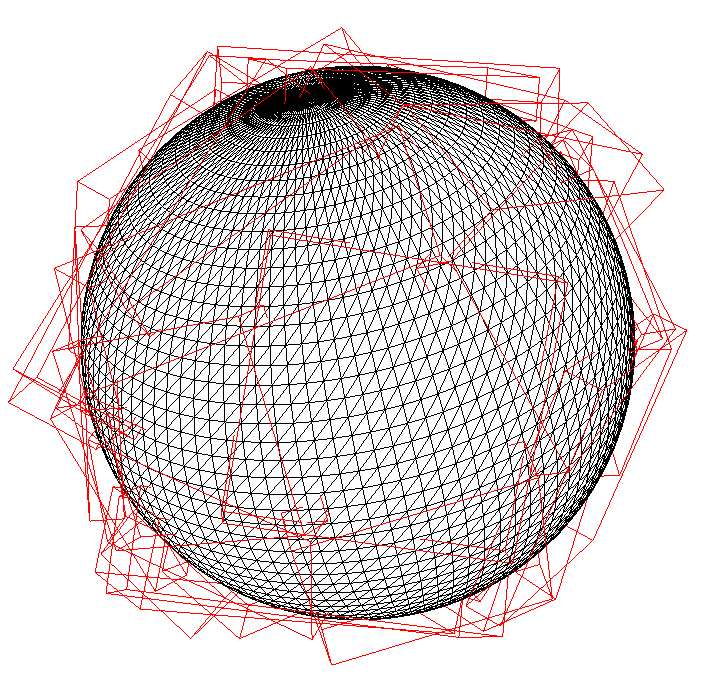
\includegraphics[width=0.4\textwidth]{./images/sphere_obbs_shallow.png}
  \end{figure}

  \column{0.1\textwidth}
  \begin{figure}
    \arrowright
  \end{figure}
  
  \column{0.45\textwidth}
  \begin{figure}
    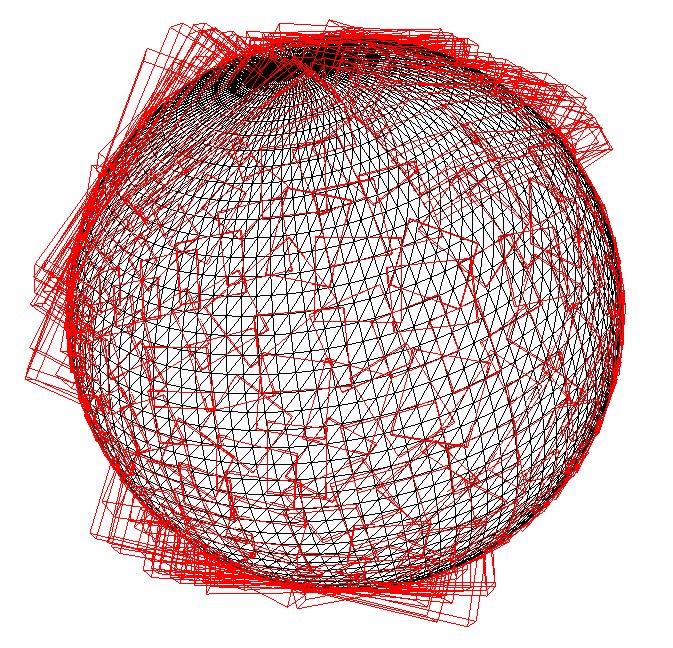
\includegraphics[width=0.4\textwidth]{./images/sphere_obbs_deep.png}
  \end{figure}
\end{columns}

\begin{itemize}
\item oriented bounding boxes are the bounding volume of choice
\item uses binary trees
\end{itemize}

\end{frame}



\begin{frame}

\frametitle{Embree's BVH}

Embree uses an OBB quad-tree structure:

\begin{center}
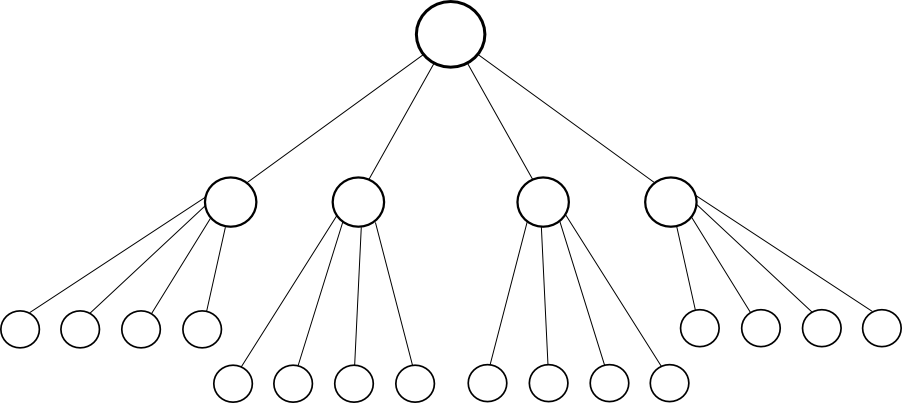
\includegraphics[width=0.5\textwidth]{./images/quad_tree.png}
\end{center}

\begin{itemize}
\item this discretizes the geometric primitives and space more finely per level in the tree
\item but it also makes for more tree nodes to check when doing a query
\item Embree makes up for this by checking many nodes at once using SIMD commands
\end{itemize}

\end{frame}


\begin{frame}
\frametitle{Embree's BVH}

\end{frame}



\section{Implementation of Embree in DAGMC} % 1-2 slides
\begin{frame}
  make\_watertight \cite{make_watertight_smith_2010} is an algorithm used to ensure the capability of robust ray tracing


  we must take care to ensure our mesh is represented in the same way in an Embree instance. 
  

\end{frame}

% Maintaining watertightness
   % explain and refer to make_watertight
% Importance of the filter functions
   % allowed compliance with DAGMC conventions
\section{Results} % 2-3 slides
% Pure ray fire comparison (no transport)
% Single volume tests
% Multiple volume tests
\section{Drawbacks} % 2-3 slides
% Floating precision 
% Robustness needs work, triangle intersector not quite there
% Lost particles in highly complex geometries, most likely due to forced conversion
% back and forth from double to float
% Extra: slide with graphic of our specific problem
\section{Future Work} % 2 slides
% Proof of principle
% Likely to see improvements in our native system using variations of these techniques
% Point them to pyembree for a simple example of a 1-D Monte Carlo calculation in 3 regions


%Citations
\begin{frame}
  \bibliographystyle{ans}
  \bibliography{bibliography}
\end{frame}

%QUESTIONS - 1 slide

\end{document}
